\documentclass[sigconf]{acmart}
\setcopyright{none}
\acmConference[]{
  Düsseldorf, NRW Deutschland}
\acmYear{}
\copyrightyear{2020}
\acmISBN{}
\acmPrice{}

%%
%% \BibTeX command to typeset BibTeX logo in the docs
\AtBeginDocument{%
  \providecommand\BibTeX{{%
    \normalfont B\kern-0.5em{\scshape i\kern-0.25em b}\kern-0.8em\TeX}}}

\begin{document}
%%
%% The "title" command has an optional parameter,
%% allowing the author to define a "short title" to be used in page headers.
\title{Unicornn: Eine Unity Sprachsteuerung}

%%
%% The "author" command and its associated commands are used to define
%% the authors and their affiliations.
%% Of note is the shared affiliation of the first two authors, and the
%% "authornote" and "authornotemark" commands
%% used to denote shared contribution to the research.
\author{Alexander Pech}
\email{alexander.pech@study.hs-duesseldorf.de}
\affiliation{%
  \institution{Hochschule Düsseldorf}
}

\author{Lara Bertram}
\email{lara.bertram@study.hs-duesseldorf.de}
\affiliation{%
  \institution{Hochschule Düsseldorf}
}

\author{Alexander Mikulaschek}
\email{alexander.mikulaschek@study.hs-duesseldorf.de}
\affiliation{%
  \institution{Hochschule Düsseldorf}
}

\author{Philipp Jonas Knohl}
\email{philipp.jonas.knohl@study.hs-duesseldorf.de}
\affiliation{%
  \institution{Hochschule Düsseldorf}
}

%%
%% The abstract is a short summary of the work to be presented in the
%% article.
\begin{abstract}
Wir präsentieren eine einfache Sprachsteuerung für die Game Engine Unity 3D. Die Sprachsteuerung erkennt einzelnen Wörter und klassifiziert diese mittels eines neuronalen Netzes. Bestimmte Kombinationen bei der Klassifizierung erlauben eine direkte zu Ordnung zu Unity-Befehlen.  
Ein Beispiel wäre der Sprachbefehl ,,Move“ + „Forward“, welcher in Unity „transform.position += Vector3.forward“ entspricht.\\
Bei dem neuronalen Netz handelt es sich um ein Convolutional Neural Network (kurz: CNN). Da diese sich gut für Klassifizierungsaufgaben eignen. Teil dieser Arbeit ist dabei auch der Performanz Vergleich zwischen VGG19 und ResNet sowie der Verwendung des SGD- und Adam-Optimizers beim Trainingsprozess. 
Zur Demonstration des Projektes wurde eine Demoscene in Unity 3D erstellt welche den Agenten enthält und es ermöglicht via Spracheingabe Objekt im Raum zu bewegen. 
\end{abstract}

%%
%% Keywords. The author(s) should pick words that accurately describe
%% the work being presented. Separate the keywords with commas.
\keywords{datasets, neural networks, speech recognition, Unity, Voice command}

%% A "teaser" image appears between the author and affiliation
%% information and the body of the document, and typically spans the
%% page.
\begin{teaserfigure}
  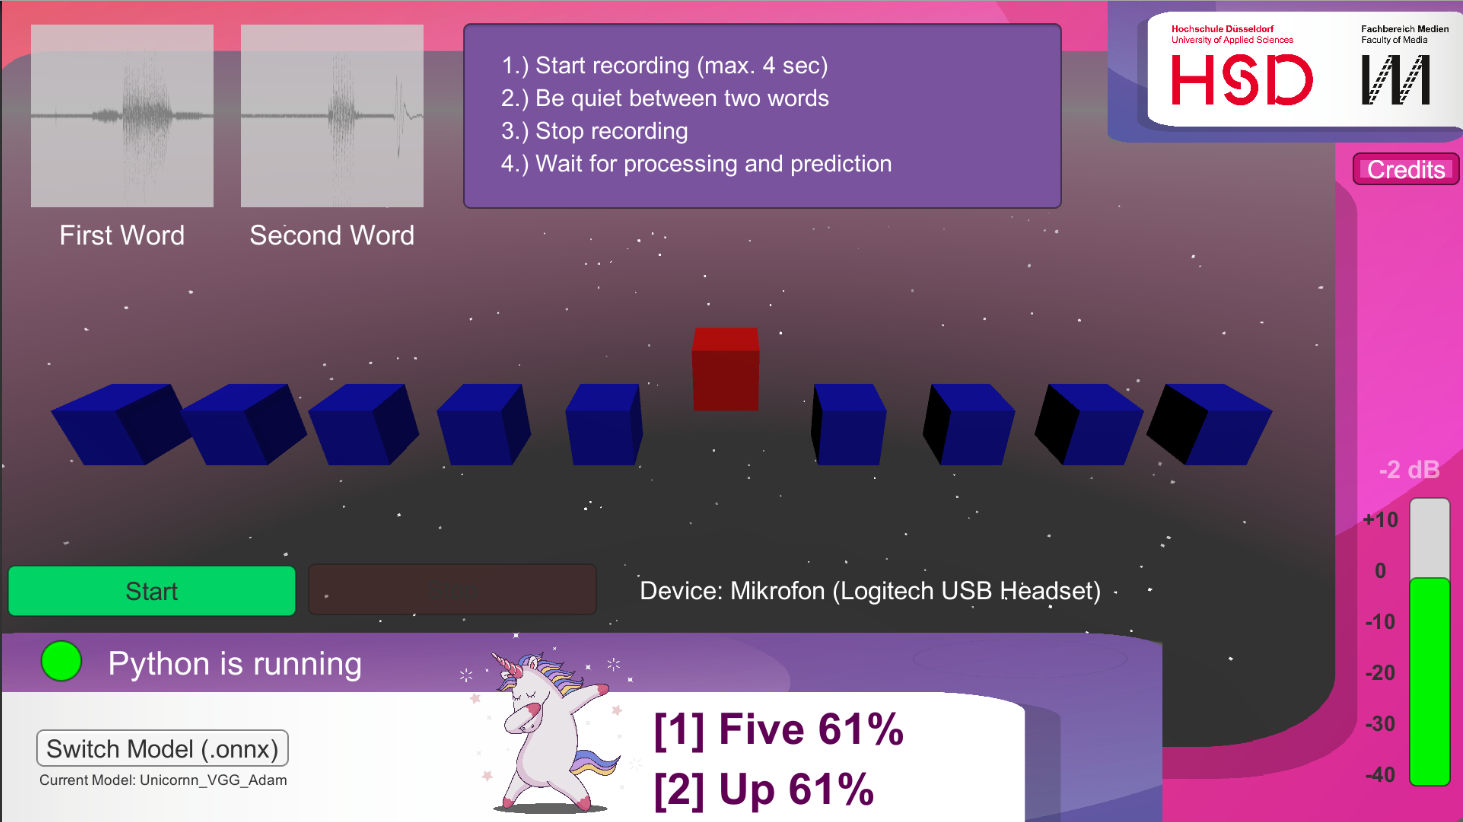
\includegraphics[width=\textwidth]{images/Demo}
  \caption{Screenshot des Interface der Unityanwendung.}
  \Description{Das Interface der Unity App.}
  \label{fig:UnityApp}
\end{teaserfigure}

%%
%% This command processes the author and affiliation and title
%% information and builds the first part of the formatted document.
\maketitle
\newpage
\section{Einleitung}

\subsection{Motivation}
Wir haben uns für dieses Projekt entschieden, da Sprachsteuerungen immer relevanter in unserem Leben werden. Zudem haben wir vorher schon viel mit Audio und GameEngines zu tun gehabt und fanden es interessant ob sich so eine Sprachsteuerung als nützlich erweisen könnte. Es war auch deshalb interessant, weil wir vorher keine Sprachassitenten in Unity oder UE4 bemerkt haben.

\subsection{Ziel}
Unser Ziel war es eine Sprachsteuerung für die GameEngine Unity zu entwickeln, mit der man einfache Sprachbefehle einsprechen kann und diese dann korrekt verarbeitet und ausgeführt werden. Unity soll imstande sein Objekte in der Szene während diese läuft zu verändern.

\section{Environment}
Möchte man den Aufbau des Projektes in Agent und Umgebung aufteilen, ist zu beachten, dass es eine Trainings- und ein Anwendungsumgebung gibt. Der Agent wird durch das CNN repräsentiert. 

\section{Trainingsumgebung}
\label{section:Umgebung}
Die Trainingsumgebung wurde in einem Jupyter-Notebook mit dem Machine Learning Framework PyTorch geschrieben. Innerhalb der Umgebung müssen zwei grundlegende Aufgaben realisiert werden. 
Die erste Aufgabe besteht darin, den Datensatz einzulesen, aufzubereiten und die Einträge mit entsprechendem Label für den Trainingsprozess bereit zu stellen. Die zweite Aufgabe ist der Trainingsprozess selbst. Detail zum Trainingsprozess werden in Kapitel~\ref{section:training} beschrieben. 

\section{Anwendungsumgebung}
Die Anwendungsumgebung in Unity stellt die Daten in demselben Format wie die Trainingsumgebung bereit. Statt die Ausgabe, wie beim Trainingsprozess,  mit Labeln zu vergleichen, werden die Ergebnisse hier interpretiert, sodass in Unity ein Befehl ausgeführt werden kann. Die Daten werden in Unity mit einem Mircrophone Input erzeugt. Die Aufnahmen werden nach Worten getrennt, wodurch es möglich ist, die Worte einzeln klassifizieren zu können. Dies ist vergleichbar damit, dass Worte im Datensatz als einzelne Dateien hinterlegt sind. 

\section{Trainings Daten}
Die Trainingsdaten stammen aus dem Speech Command Dataset v0.02 von Warden. Dieser Datensatz enthält tausende von Aufnahme einzelner Worten. Die verschiedenen Worte repräsentieren dabei die Klassen. Für unsere Anwendung sind lediglich die folgenden Worte/Aufnahmen der Klassen relevant: ,,one“, ,,two“, „three“, „four“, „five“, „six“, „seven“, ,,eight“, ,,nine“, ,,forward“, ,,backward“, „left“, „right“, „up“ und ,,down“.  

Die relevanten Daten bilden unseren Datensatz, welcher mit einem Verhältnis von 80/20 in Trainings- und Testdaten aufgeteilt wird. 
\begin{figure}[H]
  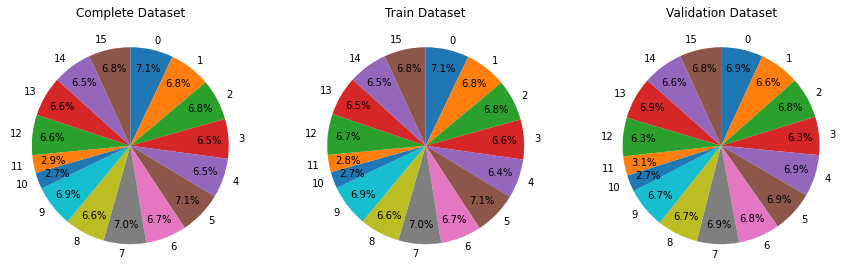
\includegraphics[width=0.45\textwidth]{images/DataBalance}
  \caption{Die verschiedenen Datensätze}
  \Description{}
  \label{fig:TrainingsDaten}
\end{figure}

Die Trainingsdaten liegen im .wav Format vor. Für die Eingabe in die Netzte werden die Aufnahmen auf eine Dauer von einer Sekunde beschränkt bzw. erweitert (hinzufügen von Stille). Bei einer Samplerate von 16kHz (mono) würde dies einer Eingabe von 16000 Werten in das Netz entsprechen. Um die Input Size zu verringern wird ein Spektrogramm der Aufnahmen erzeugt.  

Ein Vorteil der Verwendung von Spektrogrammen ist, dass es sich um eine drei dimensionale Repräsentation handelt (Zeit, Frequenz, Amplitude). Bei der Verwendung von RAW-Audio gäbe es nur die Dimensionen Zeit und Amplitude. Die dreidimensionale Repräsentation ermöglicht einen detaillierteren Einblick in die Strukturen innerhalb der Aufnahmen, die vom Netz erlernt werden sollen. 

Gespeichert werden die Spektrogramme in Form von Graustufen-Bildern (x-Ache: zeit, y-Achse: Frequenz, pixelwert: Amplitude). X und Y-Dimensionen werden dabei auf je 32 Werte beschränkt und die Amplitude wird normalisiert. 

\section{Mel-Spektrogramm}
Ein Mel-Spektrogramm ist eine Repräsentation des Kurzzeit-Energiespektrums eines Tons in Abhängigkeit des menschlichen Gehörs. Es simuliert durch Filterbänke wie das menschliche Gehör ein Geräusch wahrnimmt und hebt somit die wichtigen Frequenzen an und schwächt jene Frequenzen ab, die nicht wahrgenommen werden. 
\begin{figure}[H]
  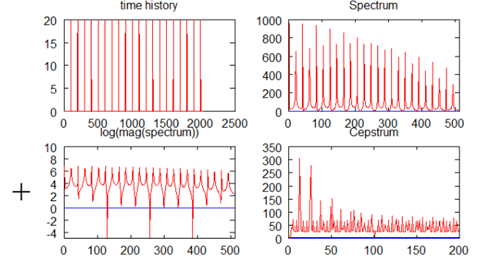
\includegraphics[width=0.45\textwidth]{images/melexplanation}
  \caption{Unterschiedliche Darstellungsmöglichkeiten von Auido}
  \Description{}
  \label{fig:TrainingsDaten}
\end{figure}
Beim Cepstrum wird auf der x-Achse die „quefrency“ dargestellt. Die Quefrenz hat als Einheit die Zeit und kann als Maß für die Verschiebung von Mustern im Zeitbereich interpretiert werden. 
\newpage
\subsection{Mel-Spektrogramm als Textur}
Das fertige Mel-Spektrogramm kann schließlich auch als eine Art Textur dargestellt werden, siehe Abb.\ref{fig:MelTextur}.  
Hier beschreibt die Farbe die Intensität, die X-Achse die Quefrenz und die Y-Achse die Frequenzbänder. 
\begin{figure}[H]
  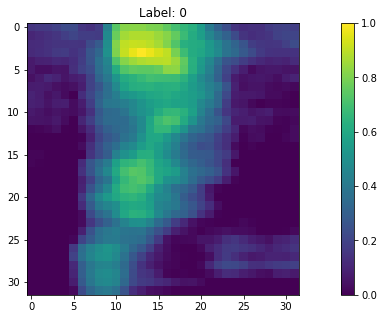
\includegraphics[width=0.45\textwidth]{images/Mel}
  \caption{Mel-Spektrogramm als Texture}
  \Description{}
  \label{fig:MelTextur}
\end{figure}

\section{Agent}
Da sich das Mel-Spektrogramm als Bild handhaben lässt, bietet sich die Verwendung von 2D-Convolutional Neural Networks an. Grundlegend lässt sich die Verarbeitung der Bilder durch CNNs in zwei Abschnitte einteilen. 

Die Feature Detection dient dazu durch zweidimensionale Faltungen markante Strukturen zu erkennen, welche für bestimmte Klassen typisch sind. Die Werte der Faltungsmatrizen werden im Training erlernt. Zur Reduzierung der Auflösung von Featuremaps wird der Maxpooling Algorithmus mit einer Kernel Größe von 2x2 (Halbierung der Auflösung) verwendet. Von 4 Pixeln wird dabei lediglich der Pixel mit dem größten Wert übernommen. Als Aktivierungsfunktion wird typischerweise die ReLu-Funktion verwendet. 

\begin{align}
ReLu(x) = \begin{Bmatrix}
f_{u}rx>0 \\
f_{u}rx \leq 0
\end{Bmatrix}
\end{align}


Die ReLu-Funktion besitzt keine Obergrenze. Um zu verhindern, das Werte im Laufe des Netzes stark gestreut werden, kommen Batch-Normalisierungs-Layer zwischen den Faltungen zum Einsatz. 
Der Klassifizierung besteht typischerweise aus vollverbundenen Schichten. Aufgabe ist es auf Basis von vielen gering aufgelösten Featuremaps (Ausgabe des ersten Abschnittes) für jede Klasse einen Score zu errechnen. Letztendlich wird sich bei der Klassenvorhersage dann für die Klasse mit dem höchsten Score entschieden. 
Für die Klassifikation wurden ein VGG19 und ein ResNet verwendet. Beim VGG handelt es sich um ein neuronales Netzwerk, bei dem die Output-Werte eines Layers als Input-Werte in das darauffolgende Layer gegeben werden. Im Unterschied dazu können bei einem ResNet vor der Eingabe dieser Werte in ein Layer noch Input-Werte vorheriger Layer aufsummiert werden, wodurch ein tieferes Netzwerk entsteht. 

\section{Training}
\label{section:training}
Beide Netze wurden über 20 Epochen trainiert. Als Loss Funktion wurde der, für Klassifizierungsprobleme oft verwendende, CrossEntropy-Loss verwendet. Der Loss-Wert wurde, bei einer Batchgröße von 128, pro Batch gemittelt.  
Um den Trainingsprozess qualitativ bewerten zu können wird nach jeder Epoche der Testdatensatz durch das Netz gespeist. Auf Basis dessen wird, neben der Berechnung eines Loss-Wertes zur Anpassung der Learningrate, überprüft, in wie vielen Fällen die Klassifizierung korrekt liegt.  Ein Accuracy-Wert von 1 repräsentiert dabei den Fall, dass die Klassifizierung für alle Testdaten erfolgreich war. Ein Wert von 0 das keine Klassifizierung korrekt war. 
Der Trainings Prozess wurde pro Netz mit dem SGD- sowie dem Adam-Optimizer durchlaufen. Letzterer führte bei beiden Netzten zu besseren Ergebnissen. Die Accuracy stieg bei beiden Netzen mit dem Adam Optimizer innerhalb von nur weniger Epochen auf über 90\%, siehe Abb. \ref{fig:VGG_Adam} und Abb. \ref{fig:ResNet_Adam}. Mit dem SGD-Optimizer konnte in keinem der beiden Netzte eine Accuracy von über 90\% innerhalb von 20 Epochen erreicht werden, siehe Abb. \ref{fig:VGG_SGD} und Abb. \ref{fig:ResNet_SGD}.

Die Learningrate war zu Beginn der Trainingsdurchläufe je 0,001. Für den Fall, dass sich der Loss-Wert für die Testdaten über 5 Epochen nicht markant ändert (<0.0001), wurde die Learningrate um den Faktor 10 verkleinert. 

\subsection{Auswertung}
Basierend auf den Loss und Accuracy-Verläufen der Testdaten im Anhang \ref{section:Anhang} schien die Verwendung des Adam-Optimizers zu besseren Ergebnissen beider Netze sowohl bei den Loss- als auch bei den Accuracy-Werten zu führen. Insgesamt schien das VGG19 Netz mit Batch Normalisierung die besten Ergebnisse liefern zu können.  

Die folgende Confusion-Matrix Abb.\ref{fig:Confusion-Matrix_VGG_Adam} zeigt die entsprechenden Ergebnisse der Testdaten. In den meisten Fällen verteilen sich alle Fehlklassifizierungen gelichmäßig auf alle anderen Klassen. Ausnahme bildet das Wort ,,four“ dies neigt bei einer Fehleinschätzung tendenziell etwas näher zur Klassifizierung als ,,forward“. Grund dafür ist mit hoher Wahrscheinlichkeit die phonetische Ähnlichkeit der beiden Worte.
\begin{figure}[H]
  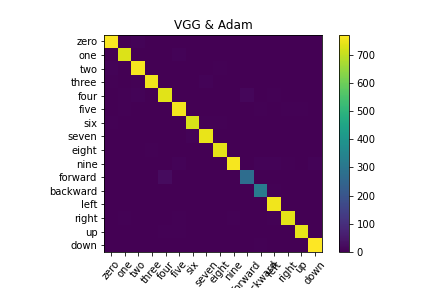
\includegraphics[width=0.4\textwidth]{images/Confusion-Matrix_VGG_Adam}
  \caption{VGG und Adam}
  \Description{}
  \label{fig:Confusion-Matrix_VGG_Adam}
\end{figure} 

\begin{figure}[H]
  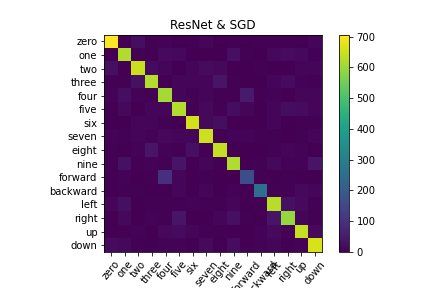
\includegraphics[width=0.4\textwidth]{images/Confusion-Matrix_ResNet_SGD}
  \caption{ResNet und SGD}
  \Description{}
  \label{fig:Confusion-Matrix_ResNet_SGD}
\end{figure} 

\begin{figure}[H]
  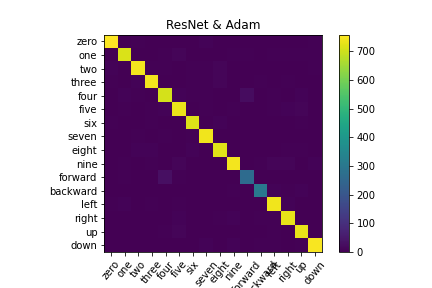
\includegraphics[width=0.4\textwidth]{images/Confusion-Matrix_ResNet_Adam}
  \caption{ResNet und Adam}
  \Description{}
  \label{fig:Confusion-Matrix_ResNet_Adam}
\end{figure} 

\begin{figure}[H]
  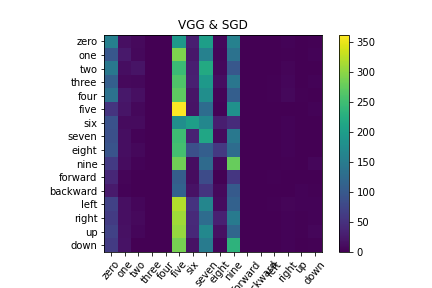
\includegraphics[width=0.4\textwidth]{images/Confusion-Matrix_VGG_SGD}
  \caption{VGG und SGD}
  \Description{}
  \label{fig:Confusion-Matrix_VGG_SGD}
\end{figure} 

Des Weiteren fällt auf, dass die Worte ,,forward“ und ,,backward“ weniger gut erkannt werden als der Rest. In Tabelle \ref{table:data} wurde bereits deutlich, dass für zwei der Klassen weniger Beispielen vorliegen. Bei diesen handelt es sich um die Worte ,,forward“ und ,,backward“ 

\begin{center}
\label{table:data}
\begin{tabular}{llll}
zero & 4052 & eight & 3787  \\
one & 3890 & nine & 3934  \\
two & 3880 & forward & 1557  \\
three &  3727 & backward & 1664 \\
four & 3728 & left & 3801 \\
five & 4052 & Right & 3779\\
six & 3860 & up & 3723\\
seven & 3998 & down & 3917 
\end{tabular}
\end{center}

Ursprünglich war eine größere Varianz an Wortkombinationsmöglichkeiten geplant. Dazu wurden bereits Sprachaufnahmen von den Worten der folgenden Wörten gesammelt: „create“, „delete“, „select“, „color“, „move“, „cube“, „sphere“, „plane“, „red“, „green“, „blue“, „white“. 

Pro Wort kamen insgesamt 147 Aufnahmen zusammen. Daraufhin war geplant diese mit Hilfe von Audio-Modulationen (u.a. Hall, Pitch, Verschiebung) zu verändern und so auf ca. 1000 Aufnahmen zu erweitern. Durch die Verwendung von zufälligen Werten bei den Modulationen sollte Korrelationen, die durch gleiche Modulations-Funktionen entstehen und zu Fehlklassifikationen führen könnten, entgegengewirkt werden.  
Dies war allerdings leider nicht genug, da man für eine möglichst genaue Vorhersage ca. 3000 Aufnahmen braucht, was man auch anhand von der Tabelle \ref{table:data} und Abb. \ref{fig:Confusion-Matrix_VGG_Adam} sehen kann.

\section{Deployment}
Mit dem Barraduca Package ist es möglich Neuronale Netz in Unity zu verwenden. Das Plugin kann Netze im eigenen Format .nn, sowie im Austauschformat .onnx einlesen und anwenden. Dabei werden noch nicht alle Funktionalitäten des ONNX-Formats komplett unterstützt. Für die Anwendung einfacher feedforward Netze ist die Komptabilität allerdings weitestgehend gegeben. Den Trainingsprozess konnten wir so mit dem Machine Learning Framework PyTorch durchführen und die Netze mit den entsprechenden Trainingständen als ONNX exportieren. Abb. \ref{fig:UnityApp} zeigt die Demo-Anwendung in Unity, welche die Anwendungsumgebung aus Kapitel \ref{section:Umgebung} darstellt. 

\subsection{Audio Slicing}
In dem Notebook “FeatureDetection” ist der Vorgang in Python umgeschrieben worden und nocheinmal deutlicher erklärt worden. In der Anwendung läuft dies über ein C\#-Script. 

Der Ablauf des Algorithmus: 
\begin{itemize}
\item Einlesen der .wav
\item Konvertieren in eine Liste aus Buffern (Custom Class)
\item Iterieren durch die Buffer-Liste und eine Serie aus "lauten" Buffern finden
\item Die Serie an "lauten" Buffern in vorhergehende und folgende Buffer einbetten
\item Die Buffer-Liste wieder in eine Float-Liste konvertieren
\end{itemize}

Man hat einige Einstellungsmöglichkeiten, mit denen man die Genauigkeit anpassen könnte. ZB. Die Größe der Buffer verringern oder den Threshhold verändern.
Dies funktioniert relativ zuverlässig und hat nur bei den Wörter "forward" und "backward" Probleme, wahrscheinlich weil dort beim Sprechen eine kleine Pause im Wort ist. Dem kann man entgegenwirken indem man die Buffersize erhöht. \\
In Abb. \ref{fig:Audio} sieht man die gesamte Audiospur und Abb. \ref{fig:Audio1} und Abb. \ref{fig:Audio2} zeigen die einzelnen getrennten Worte.
\begin{figure}[H]
  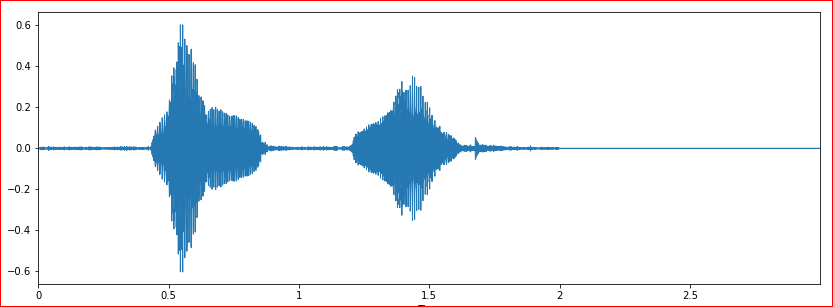
\includegraphics[width=0.3\textwidth]{images/Audio1}
  \caption{Waveform der gesamten Audiospur.}
  \Description{}
  \label{fig:Audio}
\end{figure} 
\begin{figure}[H]
  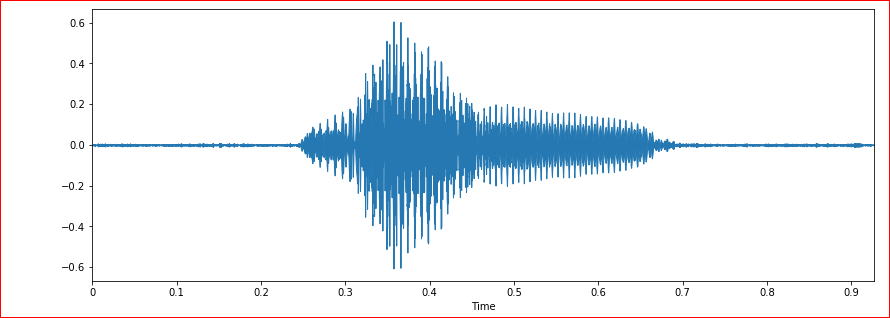
\includegraphics[width=0.3\textwidth]{images/Audio2}
  \caption{Waveform des ersten Wortes.}
  \Description{}
  \label{fig:Audio1}
\end{figure} 
\begin{figure}[H]
  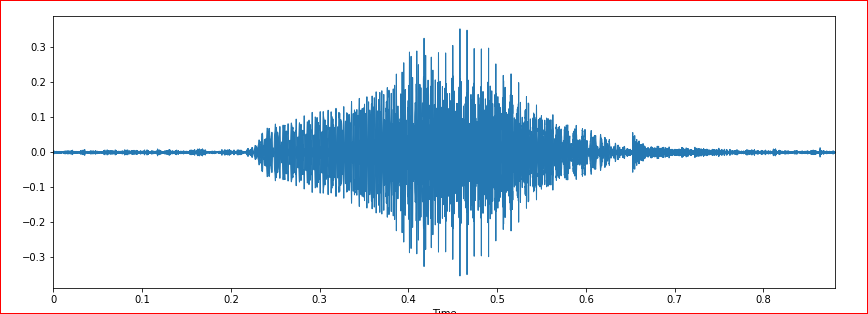
\includegraphics[width=0.3\textwidth]{images/Audio3}
  \caption{Waveform des zweiten Wortes.}
  \Description{}
  \label{fig:Audio2}
\end{figure} 
\section{Fazit}

\subsection{Zusammenfassung}
Wir haben einen Sprachassistent für Unity 3D entwickelt, der in seiner Funktionsweise derzeit noch stark begrenzt ist, dafür aber solide funktioniert. Eine Skalierung ist bei entsprechender Anzahl von Trainingsdaten durchaus denkbar. 

\subsection{Aussicht}
Derzeit wird die Spektrogramm Berechnung noch in Python durchgeführt, da in Unity 3D keine entsprechenden Funktionen bereitstehen. Der Umweg über ein Python-Script im Hintergrund kann der Zeit noch als Bottelneck der Pipline betrachtet werden und wäre für eine Auslieferung des Programms sicherlich nicht optimal. Eine Umsetzung der Daten komplett in Unity steht noch aus. 

\subsection{Conclusion}
Es ist funktioniert relativ gut einen Sprach assistenten für Unity zu entwickeln. Ein größeres Hinderniss wäre die Trainingsdatenmenge, welche nötig ist, damit die Worte richtig erkannt werden. 

\appendix
\section{Anhang}
\label{section:Anhang}
\begin{figure}[H]
  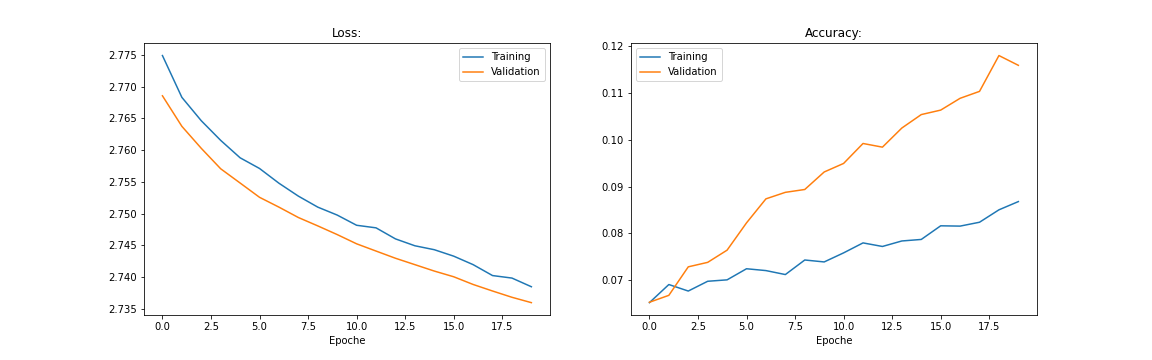
\includegraphics[width=0.45\textwidth]{images/Loss_Acc_VGG_SGD}
  \caption{Loss Accuracy von VGG \& SGD}
  \Description{}
  \label{fig:VGG_SGD}
\end{figure} 


\begin{figure}[H]
  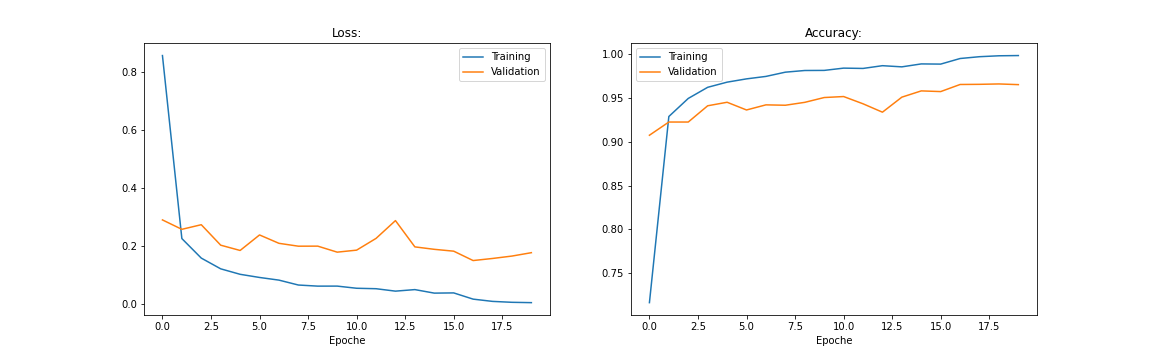
\includegraphics[width=0.45\textwidth]{images/Loss_Acc_VGG_Adam}
  \caption{Loss Accuracy von VGG \& Adam}
  \Description{}
  \label{fig:VGG_Adam}
\end{figure} 


\begin{figure}[H]
  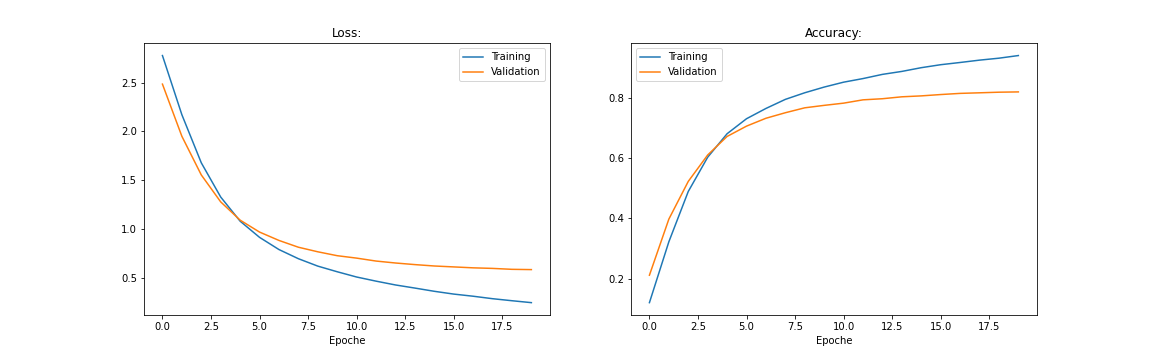
\includegraphics[width=0.45\textwidth]{images/Loss_Acc_ResNet_SGD}
  \caption{Loss Accuracy von ResNet \& SGD}
  \Description{}
  \label{fig:ResNet_SGD}
\end{figure} 


\begin{figure}[H]
  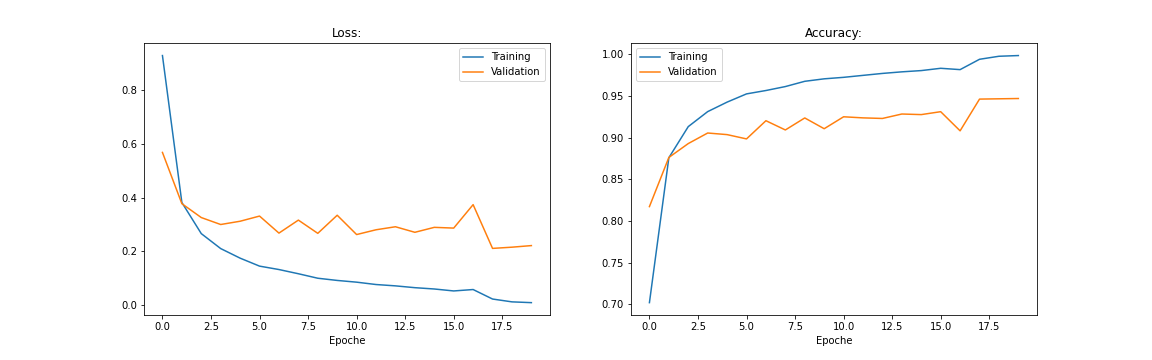
\includegraphics[width=0.45\textwidth]{images/Loss_Acc_ResNet_Adam}
  \caption{Loss Accuracy von ResNet \& Adam}
  \Description{}
  \label{fig:ResNet_Adam}
\end{figure} 

\end{document}
\endinput
